Daily customers: Gaussian Distribution\\
Normalized gaussian parameters per class (normalizing factor:1000), average and variance:

\begin{tabularx}{0.8\textwidth} { 
		| >{\raggedright\arraybackslash}X 
		| >{\centering\arraybackslash}X 
		| >{\raggedleft\arraybackslash}X | }
	\hline
	Customer Category & Average & Variance  \\
	\hline
	Category 1 & 0.15 & 0.03  \\
	\hline
	Category 2 & 0.20 & 0.03  \\
	\hline
	Category 3 & 0.40 & 0.05  \\
	\hline
	Category 4 & 0.25 & 0.04  \\
	\hline
\end{tabularx}

\begin{center}
	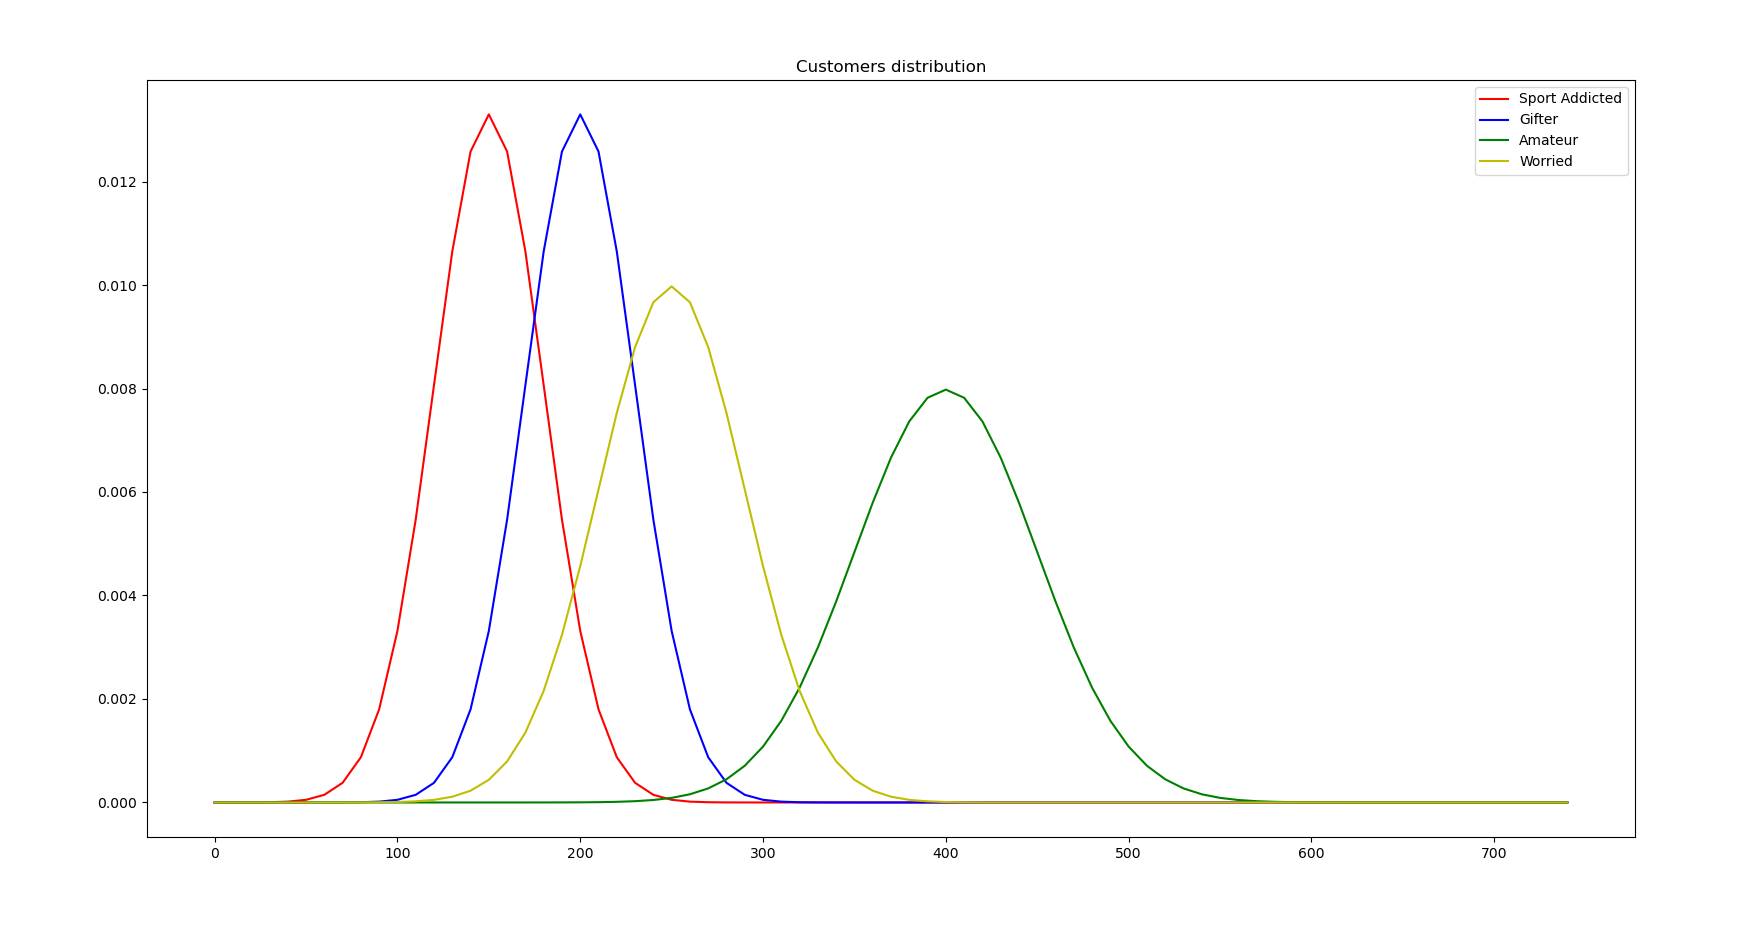
\includegraphics[scale=1]{Images/CustomerDistribution}
\end{center}


\begin{itemize}
	\item Buy item1(price) : Bernoulli \~ 0,1
	\item Buy item2(price) : Bernoulli \~ 0,1
	\item Reward item1 = buy item 1 * price item 1
	\item Reward item2 = buy item 1 * buy item 2 * price item2
	\item Time horizon = 365 days
\end{itemize}
The following graphs are the demand curves of the two item: the first three graphs are the demand curves of the first item, associated to the three seasonality (spring-summer, autumn, winter); the last three graphs are the demand curves of the second item with its respective seasonality.
\begin{center}
	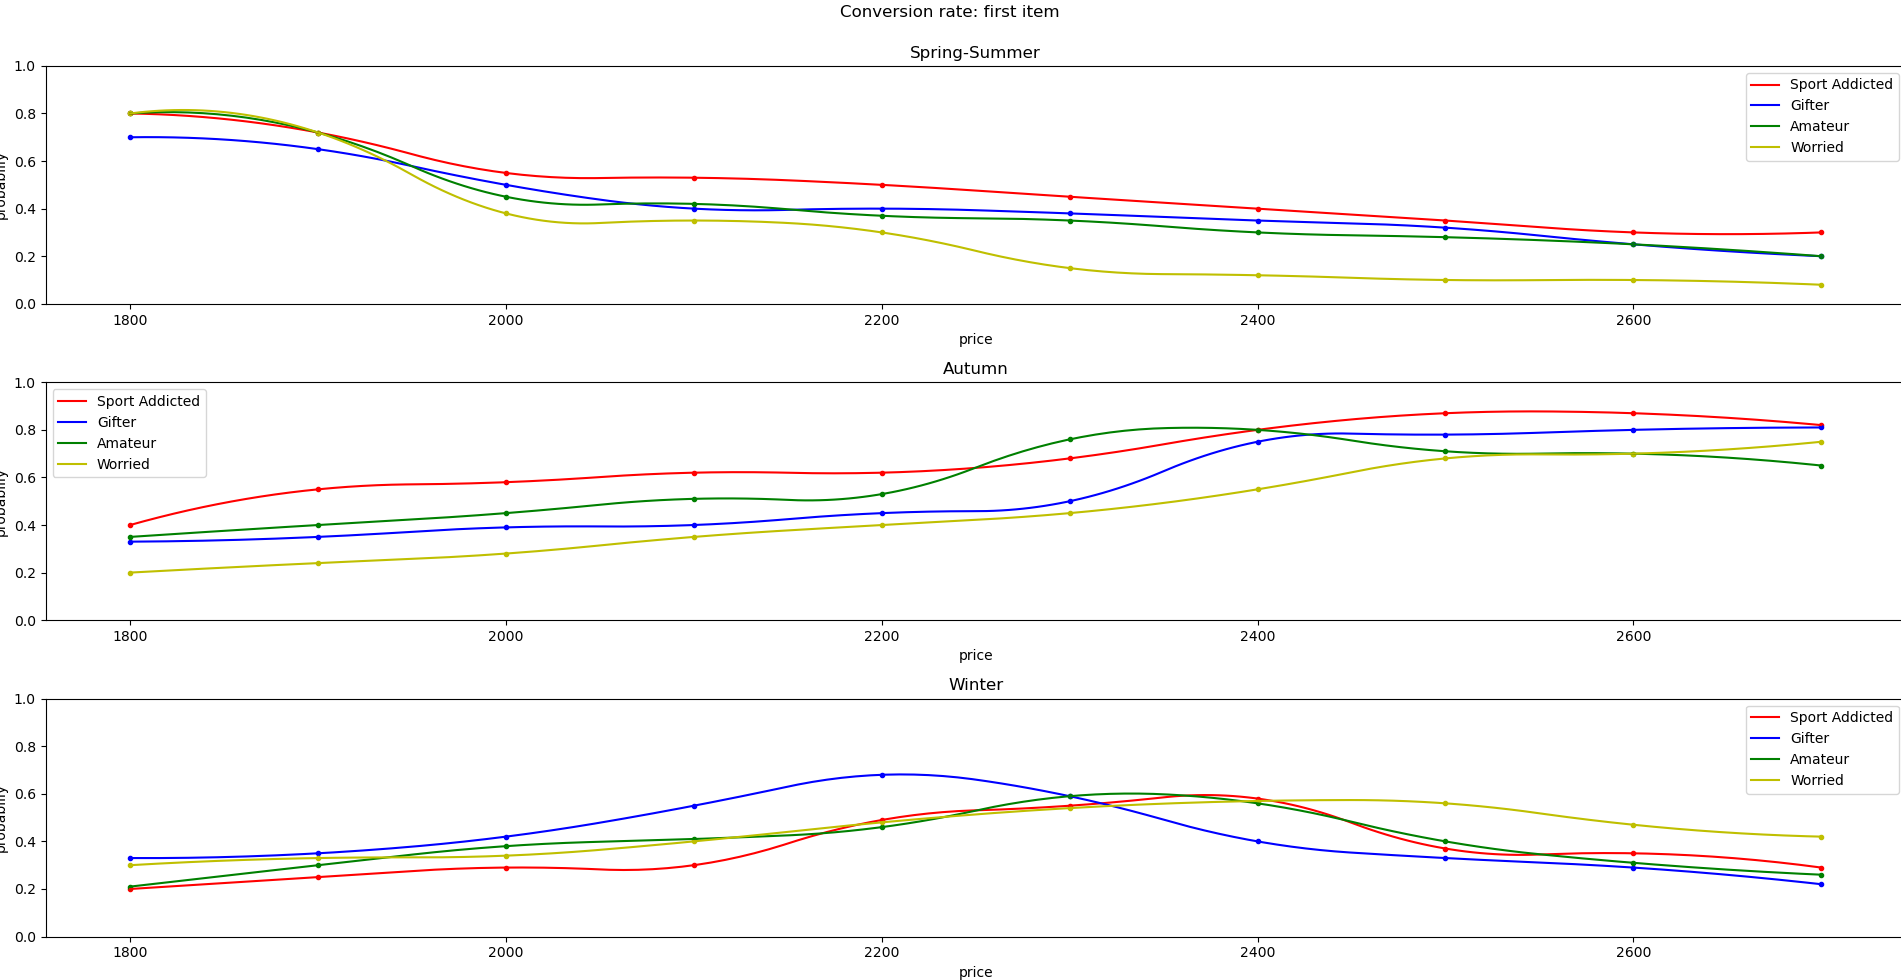
\includegraphics[scale=0.5]{Images/CR_fstItem}
\end{center}

\begin{center}
	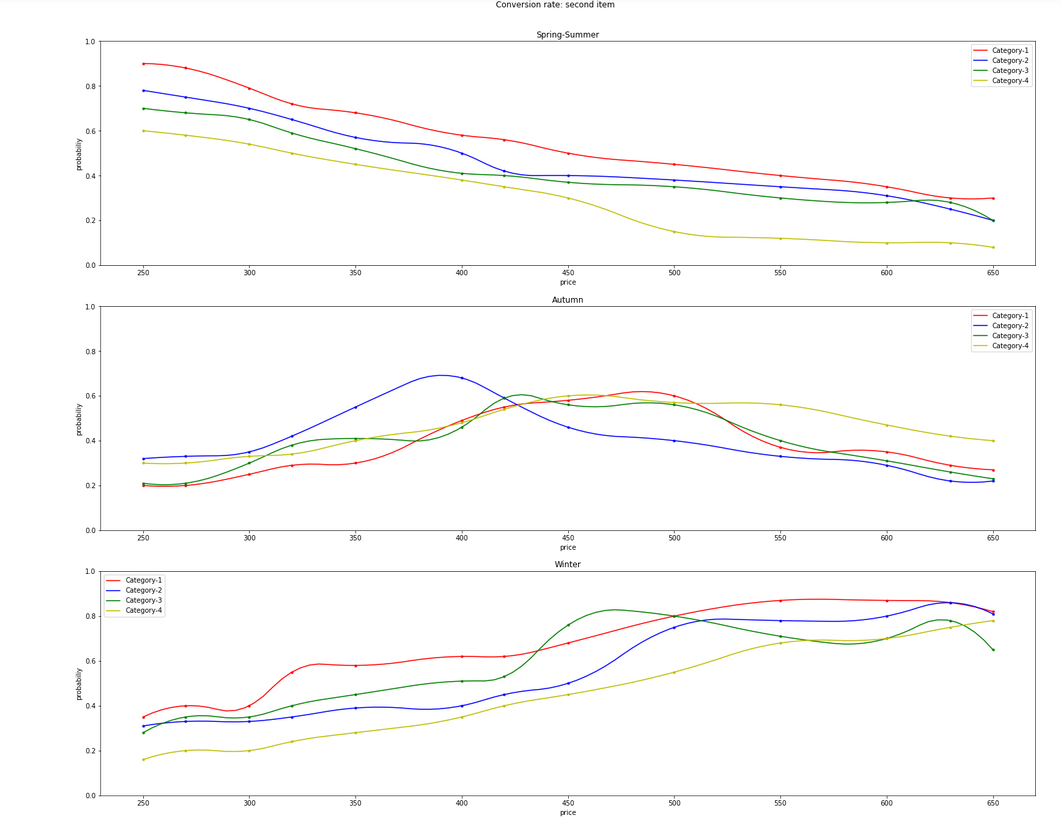
\includegraphics[scale=0.5]{Images/CR_scndItem}
\end{center}

\subsection{Online Approach}
Daily we extract the items prices using an online learner algorithm (pricing or matching), then we simulate the current day estimating the number of customers per class through the gaussian distribution. The arrival of every customer is simulated with a random approach. The system proposes the first item to every customer, simulating the purchase of it exploiting the associated Bernoulli distribution probability. The second item is proposed to the customer with the same approach, only if the first item will be bought. It is possible to exploit the information obtained in the previous steps to calculate the rewards and use them to update the learner. This procedure is repeated for every daily customer, for a time horizon of 365 days and during this period the purpose is to find a solution (composed by the prices and the assignment of promotions) that maximise the total reward. 